\section{Alpha 5}

Cette partie est une contribution personnelle dédiée à obtenir une borne de $\alpha_5$ avec l'aide de Cyril Gavoille.

\(\alpha_5 < 3.603565\)

Afin de prouver cette borne, on effectue d'abord une disjonction de cas sur la taille de l'enveloppe convexe.

On prouvera:

\begin{lemma}\label{chord}
Pour tout $P$, pour tout $\alpha >0$, on a
$$\gamma(P) \leq max(3 + chord(\alpha), 1 + 2chord(\frac{\pi}{2} - \frac{\alpha}{4})) $$
où $\gamma$ représente la longueur du chemin minimal pour un set de point P donné. et $chord$ représente la longueur d'un arc de cercle de rayon 1 et d'angle $\theta$ en particulier, $chord(\theta) = 2\sin(\theta/2)$
\end{lemma}

\begin{proof}[du théorème bidule ]
ma preuve
\end{proof}

En effet, on remarque que $3+chord(\alpha)$ est croissant et que $1 + 2chord(\frac{\pi}{2} - \frac{\alpha}{4})$ est décroissante, ainsi le minimum des deux fonctions est atteint en leur croisement qui se produit en une ordonnée $y < 3.603565$ et dont la valeur exacte n'est pas facilement calculable. Ainsi on a

\(\forall P, \gamma(P) < 3.603565\)

Ce qui montre que $\alpha_5 < 3.603565$
\newline
\newline
Dans la suite, on utilisera la notation $\gamma(T, P)$ pour donner le temps de réveil de P suivant l'arbre de réveil T.
On a alors $\forall P, \gamma(P) = \min_T(\gamma(T,P))$
et donc $\forall P, \forall T, \gamma(P) \leq \gamma(T, P)$
\subsection{Enveloppe convexe de taille 5}

Tout d'abord on tournera notre figure en sélectionnant un point tel que son axe coupe le cercle en deux demi-cercles contenant chacun 2 points. Un tel point existe toujours.

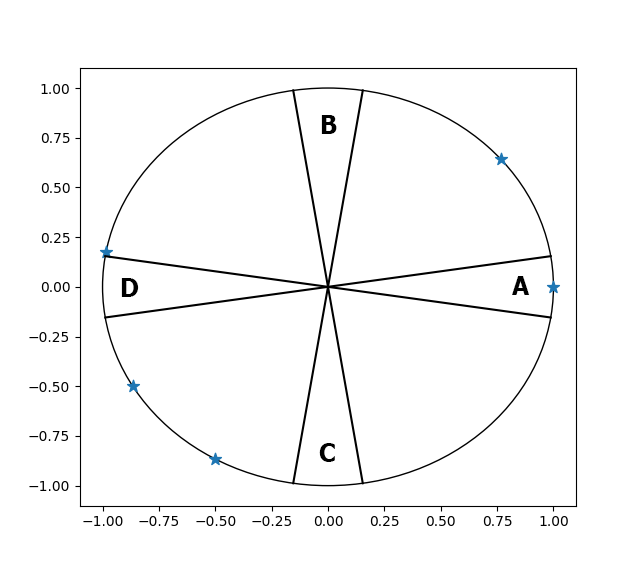
\includegraphics[scale=0.5]{initial position}

On sépare ensuite le cercle en différents cônes d'angle $\alpha$ nommés $A$, $B$, $C$, et $D$. C'est en effet ce $\alpha$ qui apparaîtra dans la formule finale. On notera $|X|$ le nombre de point dans le cône $X$ et nous ferons des disjonctions de cas sur ces derniers.

Soit $P$ un ensemble de point, on tourne le cercle comme prévu. Pour l'exemple, on positionnera les poitns sur le cercle mais les chemins utilisés marcheront quelque soit leur positionnement tant que l'enveloppe convexe est de la taille prévue.
\newline
\newline
1er cas: $\exists X, |X| \geq 2$
Dans ce cas, en réveillant les deux robots dans le cône avec celui initial, on peut aller réveiller les trois derniers où qu'ils soient dans le cercle. Réveiller les robots dans un cône d'angle $\alpha$ prend au plus un temps $1 + chord(\alpha)$ ce qui est montré dans d'autres papiers de recherche.
On peut donc réveiller tout le monde avec $\gamma(P) \leq 1 + chord(\alpha) + 2 = 3 + chord(\alpha)$
Notons que cette preuve s'applique dès que deux points sont sur un cône de taille $\alpha$ commun. On peut donc supposer désormais que cette situation n'arrive plus.
\newline
\newline
2ème cas: $|D| = 0$
On prend $T$ l'arbre commençant au noeud de $A$ et explorant de part et d'autre de son axe en commençant par le noeud le plus proche.
Soit $P'$ l'ensemble de point sur le cercle où les deux points des demi cercles sont répartis entre $A$ et $D$.
On a $\gamma(P) \leq  \gamma(T, P) \leq \gamma(T, P')$

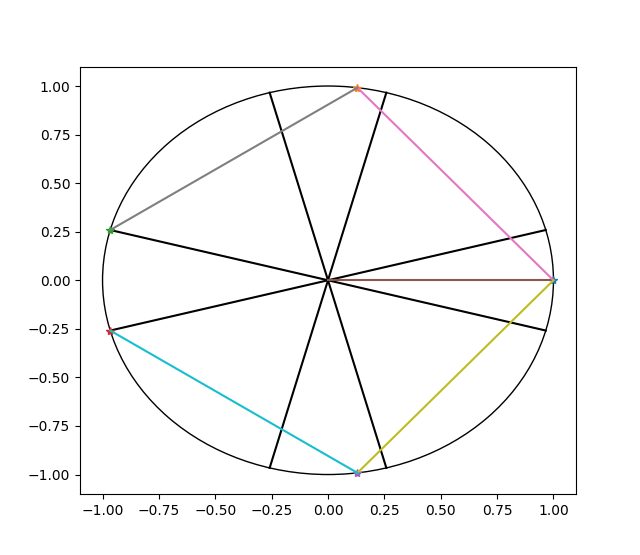
\includegraphics[scale=0.5]{2eme cas}

En effet, le pire cas pour $P$ est d'avoir un point le plus loin possible de A et d'avoir des arcs égaux, positionnant donc le dernier point du demi-cercle pile entre le point de $A$ et celui collant $D$. On a alors

$\gamma(P) \leq \gamma(T, P') = 1 + 2chord(\frac{\pi}{2} - \frac{\alpha}{4})$
\newline
\newline
3ème cas: $|B| = |C| = 0$ ($|A| = 1$ et $|D| = 1$)
Par symétrie, on peut considérer que le point dans $D$ appartient au demi-cercle du haut et donc que l'on a un seul point en haut qui ne soit pas dans $D$ que l'on nommera $b$.

-si $b$ entre $A$ et $B$ et en bas 1 point de chaque côté
on choisit pour T l'arbre commençant en bas à gauche et séparant le travail des robots en 2 comme avant.
On prend ensuite le pire cas possible pour ce T.

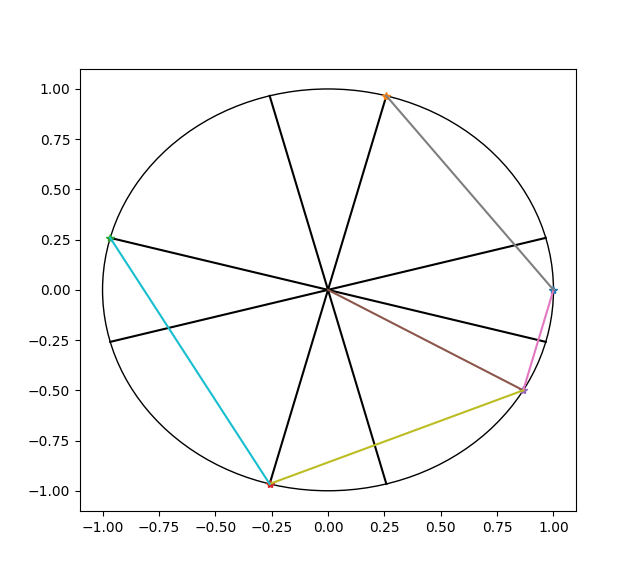
\includegraphics[scale=0.45]{3eme cas1}

En oubliant pas que l'angle entre $a$ et le point en bas à gauche est d'au moins $\alpha$ on a donc 
$\gamma(P) \leq 1 + 2chord(\frac{\pi}{2} - \frac{\alpha}{4})$

-si $b$ entre $A$ et $B$ et deux points entre $C$ et $D$
l'arbre est le suivant:

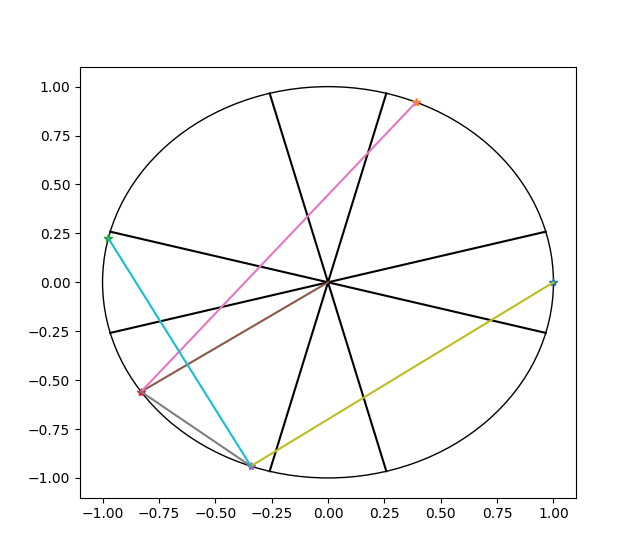
\includegraphics[scale=0.5]{3eme cas2}

$=> \gamma(P) \leq 1 + 2chord(\frac{\pi}{2} - \frac{\alpha}{4})$
-par la suite, le seul sous cas difficile est celui où $b$ entre $C$ et $D$ et les deux points du bas sont entre $A$ et $C$.
suivant l'arbre suivant:

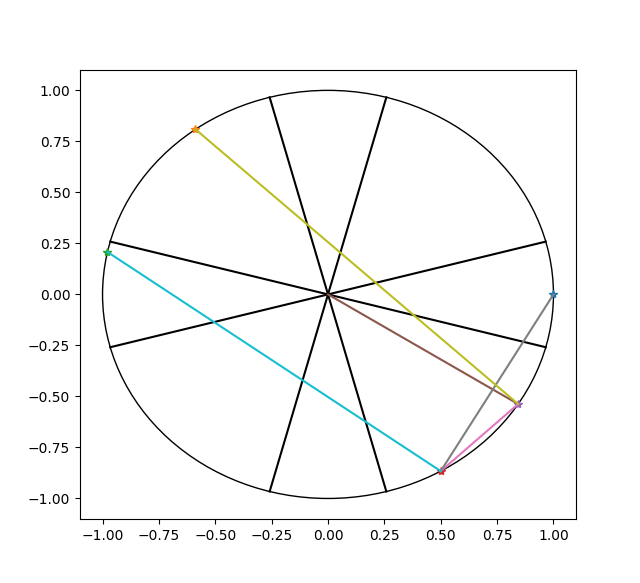
\includegraphics[scale=0.5]{3eme cas3}

on obtient alors
\(\gamma(P) \leq 1+chord(\frac{\pi}{2} - 2\alpha) + chord(\frac{\pi}{2} + \alpha) \leq 1 + 2chord(\frac{\pi}{2} - \frac{\alpha}{4})\)
\newline
\newline
4eme cas: $|A| = |B| = |C| = |D| = 1$

il reste donc un 5eme point à placer qui se trouve dans un des cônes diagonaux.

-si il est dans un cône d'angle $\alpha$ au centre du cône diagonal.

on a alors le chemin standard commençant par le 5ème point qui nous donne $\gamma(P) \leq 1 + 2chord(\frac{\pi}{2} - \frac{\alpha}{4})$

-si ca n'est pas le cas alors on prend l'arbre suivant

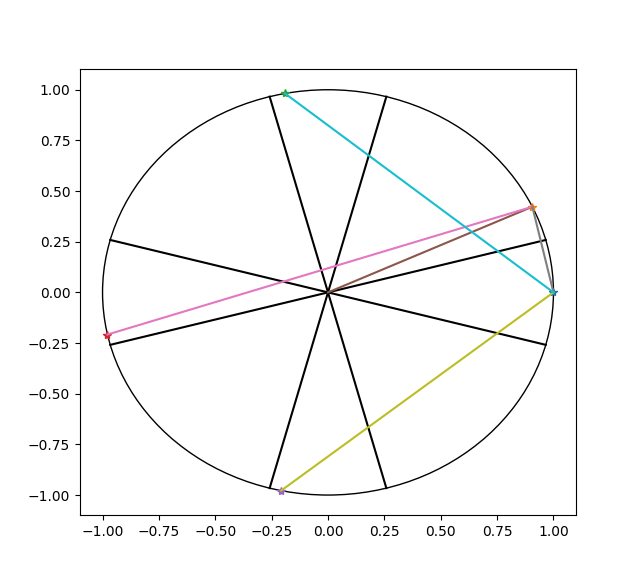
\includegraphics[scale=0.5]{4eme cas}

on a donc $\gamma(P) \leq 1 + chord(\frac{\pi}{4}) + chord(\frac{\pi}{2} + \alpha) \leq max(3 + chord(\alpha), 1 + 2chord(\frac{\pi}{2} - \frac{\alpha}{4}))$
\newline
\newline
5ème cas: $|B| = |A| = |D| = 1, |C| = 0$
à noter que par symétrie, ca s'applique pour $|B| = 0$ et $|C| = 1$

Si le point dans D appartient au demi-cercle du haut:

-Si en bas il y a un point de chaque côté, on choisit le point en bas qui se trouve du côté de B et on termine de façon standard. On a alors $\gamma(P) \leq 1 + 2chord(\frac{\pi}{2} - \frac{\alpha}{4})$

-si en bas on a les deux points du même côté, on commence par celui au milieu des deux points qui le collent pour obtenir le même résultat.

Si le point dans D appartient au demi-cercle du bas, alors commencer par $b$ ou le point libre du haut solutionnera toujours le problème...

\subsection{convexe de taille 4 ou 3}

Désormais, il faut terminer avec les cas où l'enveloppe convexe est de taille 3 ou 4. Heureusement, ces cas sont plus simples.
Si l'enveloppe convexe est de taille 3, on va vers le point le plus proche du centre qui soit à l'intérieur de l'enveloppe convexe, ensuite un des deux robots ira chercher le deuxième point à l'intérieur tandis que le deuxième ira réveiller le point le plus proche du triangle avant d'aller sur les deux autres.

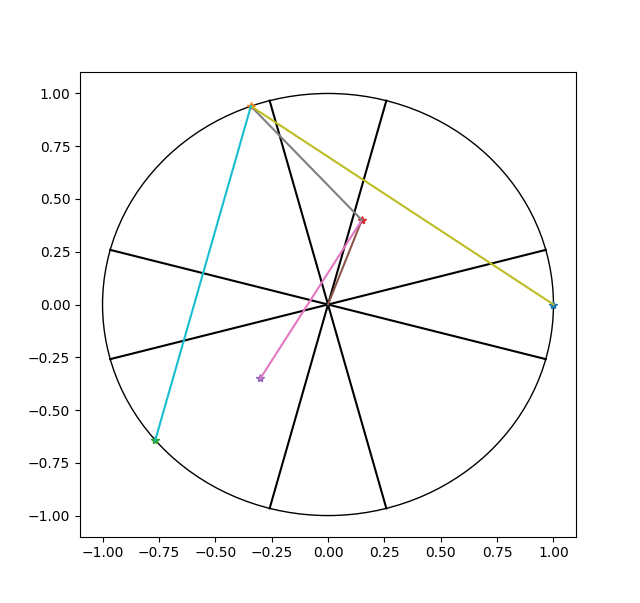
\includegraphics[scale=0.5]{n3}

En effet, le pire cas est si le point que l'on rejoint en premier est projeté sur l'enveloppe convexe orthogonalement ce qui nous donne $\exists \theta, \gamma(P) \leq \cos(\theta) + \sin(\theta) + 2 \leq \sqrt{2} + 2 \leq max(3 + chord(\alpha), 1 + 2chord(\frac{\pi}{2} - \frac{\alpha}{4}))$

Note: En réalité, cela fonctionne quelque soit l'emplacement du deuxième point à l'intérieur, et donc également si il n'est pas dans l'enveloppe connexe, et il est donc possible de traiter par exactement la même méthode le cas où l'enveloppe convexe est de taille 4.

Ainsi, on a montré le résultat voulu et par une analyse graphique, on obtient $\alpha$ tel que $\gamma(P)$ soit minimal. L'équation ne se résolvant pas facilement, on approxime et augmente la valeur pour obtenir \(\alpha_5 < 3.603565\)